\documentclass{report}

%\usepackage{times}
%\usepackage[pdftex,
%  colorlinks=true,
%  pdfstartview=FitV,
%  linkcolor=blue,
%  citecolor=blue,
%  urlcolor=blue]{hyperref}
\usepackage{geometry}
\geometry{a4paper}
\usepackage{amssymb}
%\usepackage{epstopdf}
\usepackage{xspace}
\usepackage{indentfirst}
\usepackage{float}

\usepackage[francais]{babel}
\usepackage[latin1]{inputenc}
\usepackage[dvips]{graphicx}
\usepackage{array}
\usepackage{multirow}
\usepackage{fancyheadings}
\usepackage[Lenny]{fncychap}
\pagestyle{fancy}
\newcommand{\sauteligne}{\vspace{0.5cm}}
\newcommand{\visidia}{ViSiDiA\xspace}
\newcommand{\berlios}{BerliOs.de\xspace}
\author{}
\date{}

\title{
  \begin{flushright}
    \begin{Huge}
      \begin{textbf}
        Projet \visidia\\
      \end{textbf}
    \end{Huge}
    \rule{\textwidth}{2mm}\\
    \large\rm{Cahier des charges}\\
    \vspace{2cm}
    \begin{textbf}\\
      \underline{Auteurs} :\\
      \vspace{0.5cm}
      \sc
      Ammar Aymen\\
      Balan Alexandre\\
      Ben Alaya Ramzi\\
      Bochu Fabien\\
      Bonin �ric\\
      Lafon Julien\\
      \vspace{5mm}
    \end{textbf}
    \rm 9 f�vrier 2007
  \end{flushright}
}

\begin{document}
\maketitle
\tableofcontents

\chapter{Introduction et motivation}

L'algorithmique  distribu�e  devient de  nos  jours  de  plus en  plus
importante au vu des utilisations  possibles sur les r�seaux et autres
syst�mes distribu�s.\\

Cependant,  les  algorithmes  qui   en  d�coulent  sont  difficiles  �
impl�menter, tester et exp�rimenter. C'est dans le but de faciliter la
t�che �  un utilisateur humain que  \visidia a �t� cr��  (voir le site
internet   \cite{visidiaLaBRI}).   Ce   logiciel  a   pour  principale
caract�ristique  de  permettre  la  visualisation,  au  travers  d'une
animation  graphique en  temps  r�el, de  l'ex�cution d'un  algorithme
distribu� sur un graphe donn�.   Cet algorithme peut �tre choisi parmi
une liste, d�velopp� par l'utilisateur ou encore dessin�
gr�ce � des r�gles de r��criture.\\

\visidia  se compose aujourd'hui  de trois  couches. Tout  d'abord une
interface  graphique qui  permet �  l'utilisateur d'interagir  avec le
programme. Elle  permet de cr�er  des r�seaux (graphes)  et d'ex�cuter
des algorithmes  distribu�s afin de  les tester avec  visualisation ou
non. Ensuite, une biblioth�que de  fonctions de haut niveau qui permet
de d�finir des algorithmes distribu�s (envoi, r�ception, traitement de
messages etc...).  Enfin, un simulateur dont le but est de faire le
pont entre les deux autres parties : c'est le centre de \visidia.\\

Les  fonctionnalit�s   que  proposent   \visidia  sont  tout   �  fait
int�ressantes. Malheureusement, l'implantation  actuelle ne permet pas
de faire des tests sur de gros graphes (avec plus de 20 000 noeuds) ce
qui a amen� les chercheurs du LaBRI charg�s de ce projet � proposer un
sujet de  projet de fin d'ann�e �  l'ENSEIRB. Le PFA est  un module de
quatri�me semestre  d'informatique et a pour but  de nous familiariser
avec les m�thodes de travail en  groupe sur des projets de plus longue
dur�e et de plus grande taille que ceux dont nous avons
l'habitude.\\

Notre  but au  cours  des mois  qui  vont suivre  est  de fournir  une
extension  au logiciel.   Cette extension  aura pour  r�le  d'offrir �
l'utilisateur les outils (analogues � ceux existants d�j�) n�cessaires
� l'ex�cution d'algorithmes distribu�s � l'aide d'agents mobiles.\\

Les d�finitions de la notion d'agent mobile sont nombreuses c'est pour
cela  que nous  devons nous  tenir  � le  d�finition plus  restrictive
donn�e par  les clients.  Dans le  cadre de \visidia,  un agent mobile
sera donc une entit� autonome de  calcul qui se d�place dans le graphe
et agit  sur les  noeuds en fonction  de l'algorithme �  ex�cuter. Une
bonne  r�f�rence concernant  ce type  d'agent pourra  se  trouver dans
\cite{agentBook}.

L'implantation  des  agents mobiles  dans  \visidia permettra,  ainsi,
d'augmenter   ses  capacit�s   de  simulation.    Les   deux  m�thodes
(algorithmique  distribu�e  classique  ou  par agents  mobiles)  �tant
�quivalentes d'un point de vue th�orique on pourra alors �crire et
ex�cuter les algorithmes avec la m�thode de notre choix.\\

Le  lecteur  pourra se  r�ferrer  aux  articles \cite{bauderon01a}  et
\cite{bauderon01b}  pour plus  d'informations sur  \visidia. Consultez
aussi    le    site    internet    officiel   du    projet    \visidia
\cite{visidiaLaBRI}.

A inserer :
\cite{labri} \cite{enseirb}

%% Local Variables:
%% mode: latex
%% coding: latin-1
%% TeX-master: "main"
%% End:
\chapter{Mod�le du syst�me}



\section{Cas d'utilisation}




\section{Diagramme de classes}

\begin{figure}
  \centering
  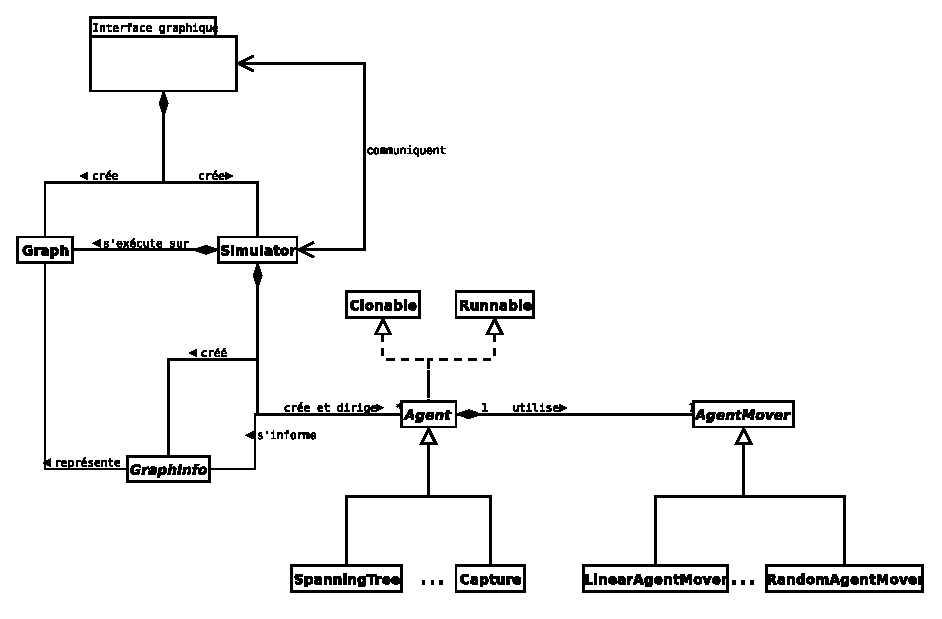
\includegraphics[width=15cm]{figures/classes}  
  \caption{Diagramme de classes}
\end{figure}


%% Local Variables:
%% mode: latex
%% coding: latin-1
%% TeX-master: "main"
%% End:
Dans  cette partie  nous d�crirons  les besoins  fonctionnels  li�s au
projet  (A.P.I,  interface) ainsi  que  les  besoins non  fonctionnels
(langage, licence, etc).


\section{Description de l'A.P.I}
\label{sec:api}

Les m�thodes de la classe \emph{Agent} fournies � l'utilisateur pour
l'�criture de l'algorithme sont les suivantes :\\

\begin{description}

\item[getArity]  retourne  le nombre  de  portes  sortantes du  sommet
  courant (la premi�re est num�rot�e 0)
\item[getVertexIdentity] retourne le num�ro du sommet courant (suppose
  que l'algorithme utilise un identifiant unique pour chaque sommet) %
\item[getNetSize] retourne le nombre de sommets du graphe %
\item[setAgentMover]  permet de  d�finir pour  l'agent un  nouveau  type de
d�placement dont le nom est pass� en param�tre %
\item[getAgentMover] retourne le type de d�placement utilis� par
l'agent %
\item[move] permet de d�placer l'agent sur la porte suivante ou sur la
  porte dont le num�ro est pass� en param�tre %
\item[moveToDoor] permet de d�placer l'agent sur la porte pass�e en
param�tre. M�thode de bas niveau. La m�thode move() associ�e � un
AgentMover est de plus haut niveau %
\item[moveBack] permet de d�placer l'agent sur la porte dont il vient %
\item[entryDoor] retourne  le num�ro de la porte  par laquelle l'agent
  vient d'arriver %
\item[getIdentity] retourne l'identifiant unique de l'agent %
\item[setProperty] place une propri�t� sur le tableau blanc de
  l'agent, la valeur et la cl� sont pass�es en param�tre %
\item[getProperty] retourne la valeur de la propri�t� du tableau blanc
  dont la cl� est pass�e en param�tre %
\item[getPropertyKeys] retourne une collection de toutes les cl�s du
tableau blanc de l'agent%
\item[lockVertexProperties] verrouille le tableau blanc du sommet
courant. Si le sommet est d�j� verrouill�, attend jusqu'� ce que le
propri�taire d�verrouille le sommet %
\item[unlockVertexProperties] d�verrouille le tableau blanc du sommet
courant %
\item[vertexPropertiesLocked] retourne vrai si le sommet est
verrouill�, faux sinon %
\item[lockVertexIfPossible] verrouille le tableau blanc du sommet
courant si possible et retourne vrai. Retourne faux sinon %
\item[getVertexPropertiesOwner] retourne l'Agent qui verrouille le
tableau blanc du sommet courant ou null si aucun Agent ne bloque le
sommet %
\item[getVertexProperty] retourne la valeur de la propri�t� du tableau blanc
  du sommet courant dont la cl� est pass�e en param�tre %
\item[setVertexProperty] place une propri�t� sur le tableau blanc du
sommet courant, la valeur et la cl� sont pass�es en param�tre %
\item[getVertexPropertyKeys] retourne une collection de toutes les cl�s du
tableau blanc du sommet courant %
\item[changeDoorState] change l'�tat de l'arr�te associ�e � la porte
pass�e en param�tre sur le sommet courant %
\item[markDoor] marque l'arr�te associ�e � la porte pass�e en
param�tre en gras %
\item[unmarkDoor] annule l'effet de markDoor() %
\item[getDoorProperty] retourne la valeur  de la propri�t� dont la cl�
  est pass�e en  param�tre, sur la porte dont  le num�ro est �galement
  pass� en param�tre
\item[cloneAgent] clone l'agent. Cr�e un nouvel Agent de m�me type sur
le sommet courant %
\item[cloneAndSend] clone l'agent en cours et envoie le clone sur la
  porte pass�e en param�tre %
\item[createAgent] cr�e un nouvel agent sur le sommet courant du type
pass� en param�tre %
\item[createAgentAndSend] est � createAgent() ce que cloneAndSend()
est � cloneAgent() %
\item[className] retourne le nom de la classe dont l'agent est une
instance sous la forme d'une cha�ne de caract�res %
\item[sleep] endort l'agent pendant le temps en milisecondes pass� en
param�tre %
\item[death] tue l'agent. Il est conseill� de sortir de la m�thode
init() pour tuer un agent plut�t que d'utiliser cette m�thode %
\item[newPulse] informe le simulateur qu'un SynchronizedAgent commence
un nouveau tour %
\item[incrementStat] incr�mente la cl� du tableau blanc pass�e en
param�tre. M�thode utile dans le cadre de la collecte de statistiques
\\

\end{description}

Il sera ainsi possible de cloner un \emph{agent}, et �ventuellement de
l'envoyer sur  une porte. L'\emph{agent}, ainsi cr��,  pourra avoir un
type de d�placement, ainsi qu'un  algorithme diff�rents de ceux de son
p�re.\\

Les  \emph{agents}  auront  �galement  d'autres  fonctionnalit�s,  ils
doivent  notamment   pouvoir  se  rencontrer,   c'est-�-dire,  pouvoir
d�tecter qu'un  autre \emph{agent} est sur  le m�me sommet,  ou sur la
m�me ar�te. Cela  va imposer la mise en place  de r�gles de priorit�s,
pour que  plusieurs \emph{agents}  ne puissent pas  agir simultan�ment
sur un m�me sommet.\\

Enfin,  les agents  pourront, s'ils  le souhaitent,  faire appel  � un
syst�me de synchronisation afin d'effectuer des actions et se d�placer
de mani�re coordonn�e.\\

L'initialisation  des objets  se fera  au plus  tard. En  effet,  ils ne
seront initialis�s, que lorsqu'ils  seront utilis�s. Pour les tableaux
blancs des  sommets, notamment, leur  initialisation ne se  fera qu'au
passage d'un \emph{agent}, s'il celui-ci souhaite lire une valeur.

\section {Interface}

Notre  graphe  pourra d�buter  avec  autant  d'agent  que le  souhaite
l'utilisateur, tous les agents n'�tant pas forc�ment du m�me type.\\

L'utilisateur aura diff�rentes possibilit�s pour placer ses agents :\\

\begin{itemize}

\item \textbf{A la  souris : } L'utilisateur choisit  un type d'agent,
et le place  sur les sommets o� il souhaite  faire d�marrer les agents
de ce type.   Il peut ensuite choisir d'autres  types d'agent pour les
placer sur les sommets restants.\\

\item \textbf{Par fichier :  } L'utilisateur cr�e un fichier contenant
l'identifiant de chaque sommet o�  il souhaite voir d�marrer un agent,
auquel  il rattache  un type  d'agent.  Cela  revient au  m�me  que la
m�thode � la souris, mais est indispensable pour les graphes de grande
taille.\\

\item \textbf{Al�atoire  : } L'utilisateur choisit un  type d'agent et
un nombre d'agents (1,2,...,*).  Le logiciel se charge alors  de r�partir ce
ou ces  agents de  fa�on al�atoire sur  les sommets du  graphe.  Cette
m�thode pourrait �tre int�ressante pour tester des algorithmes de type
policiers/voleur, avec plusieurs agents essayant d'en encercler un.
On souhaite �galement donner la possibilit� � l'utilisateur de
sp�cifier un algorithme de placement des agents (en affectant, par
exemple, � chaque sommet une probabilit� d'y placer un agent).
\end{itemize}

\section{Diagrammes de s�quences}

Nous d�crirons dans cette  section quelques sc�narios possibles durant
la vie d'un agent.

\subsection{D�placement}

Figure  \ref{fig:diagramme_seqDeplacement} :  Sc�nario  de d�placement
d'un agent sur le graphe.

\begin{figure}[h!t]
  \centering
  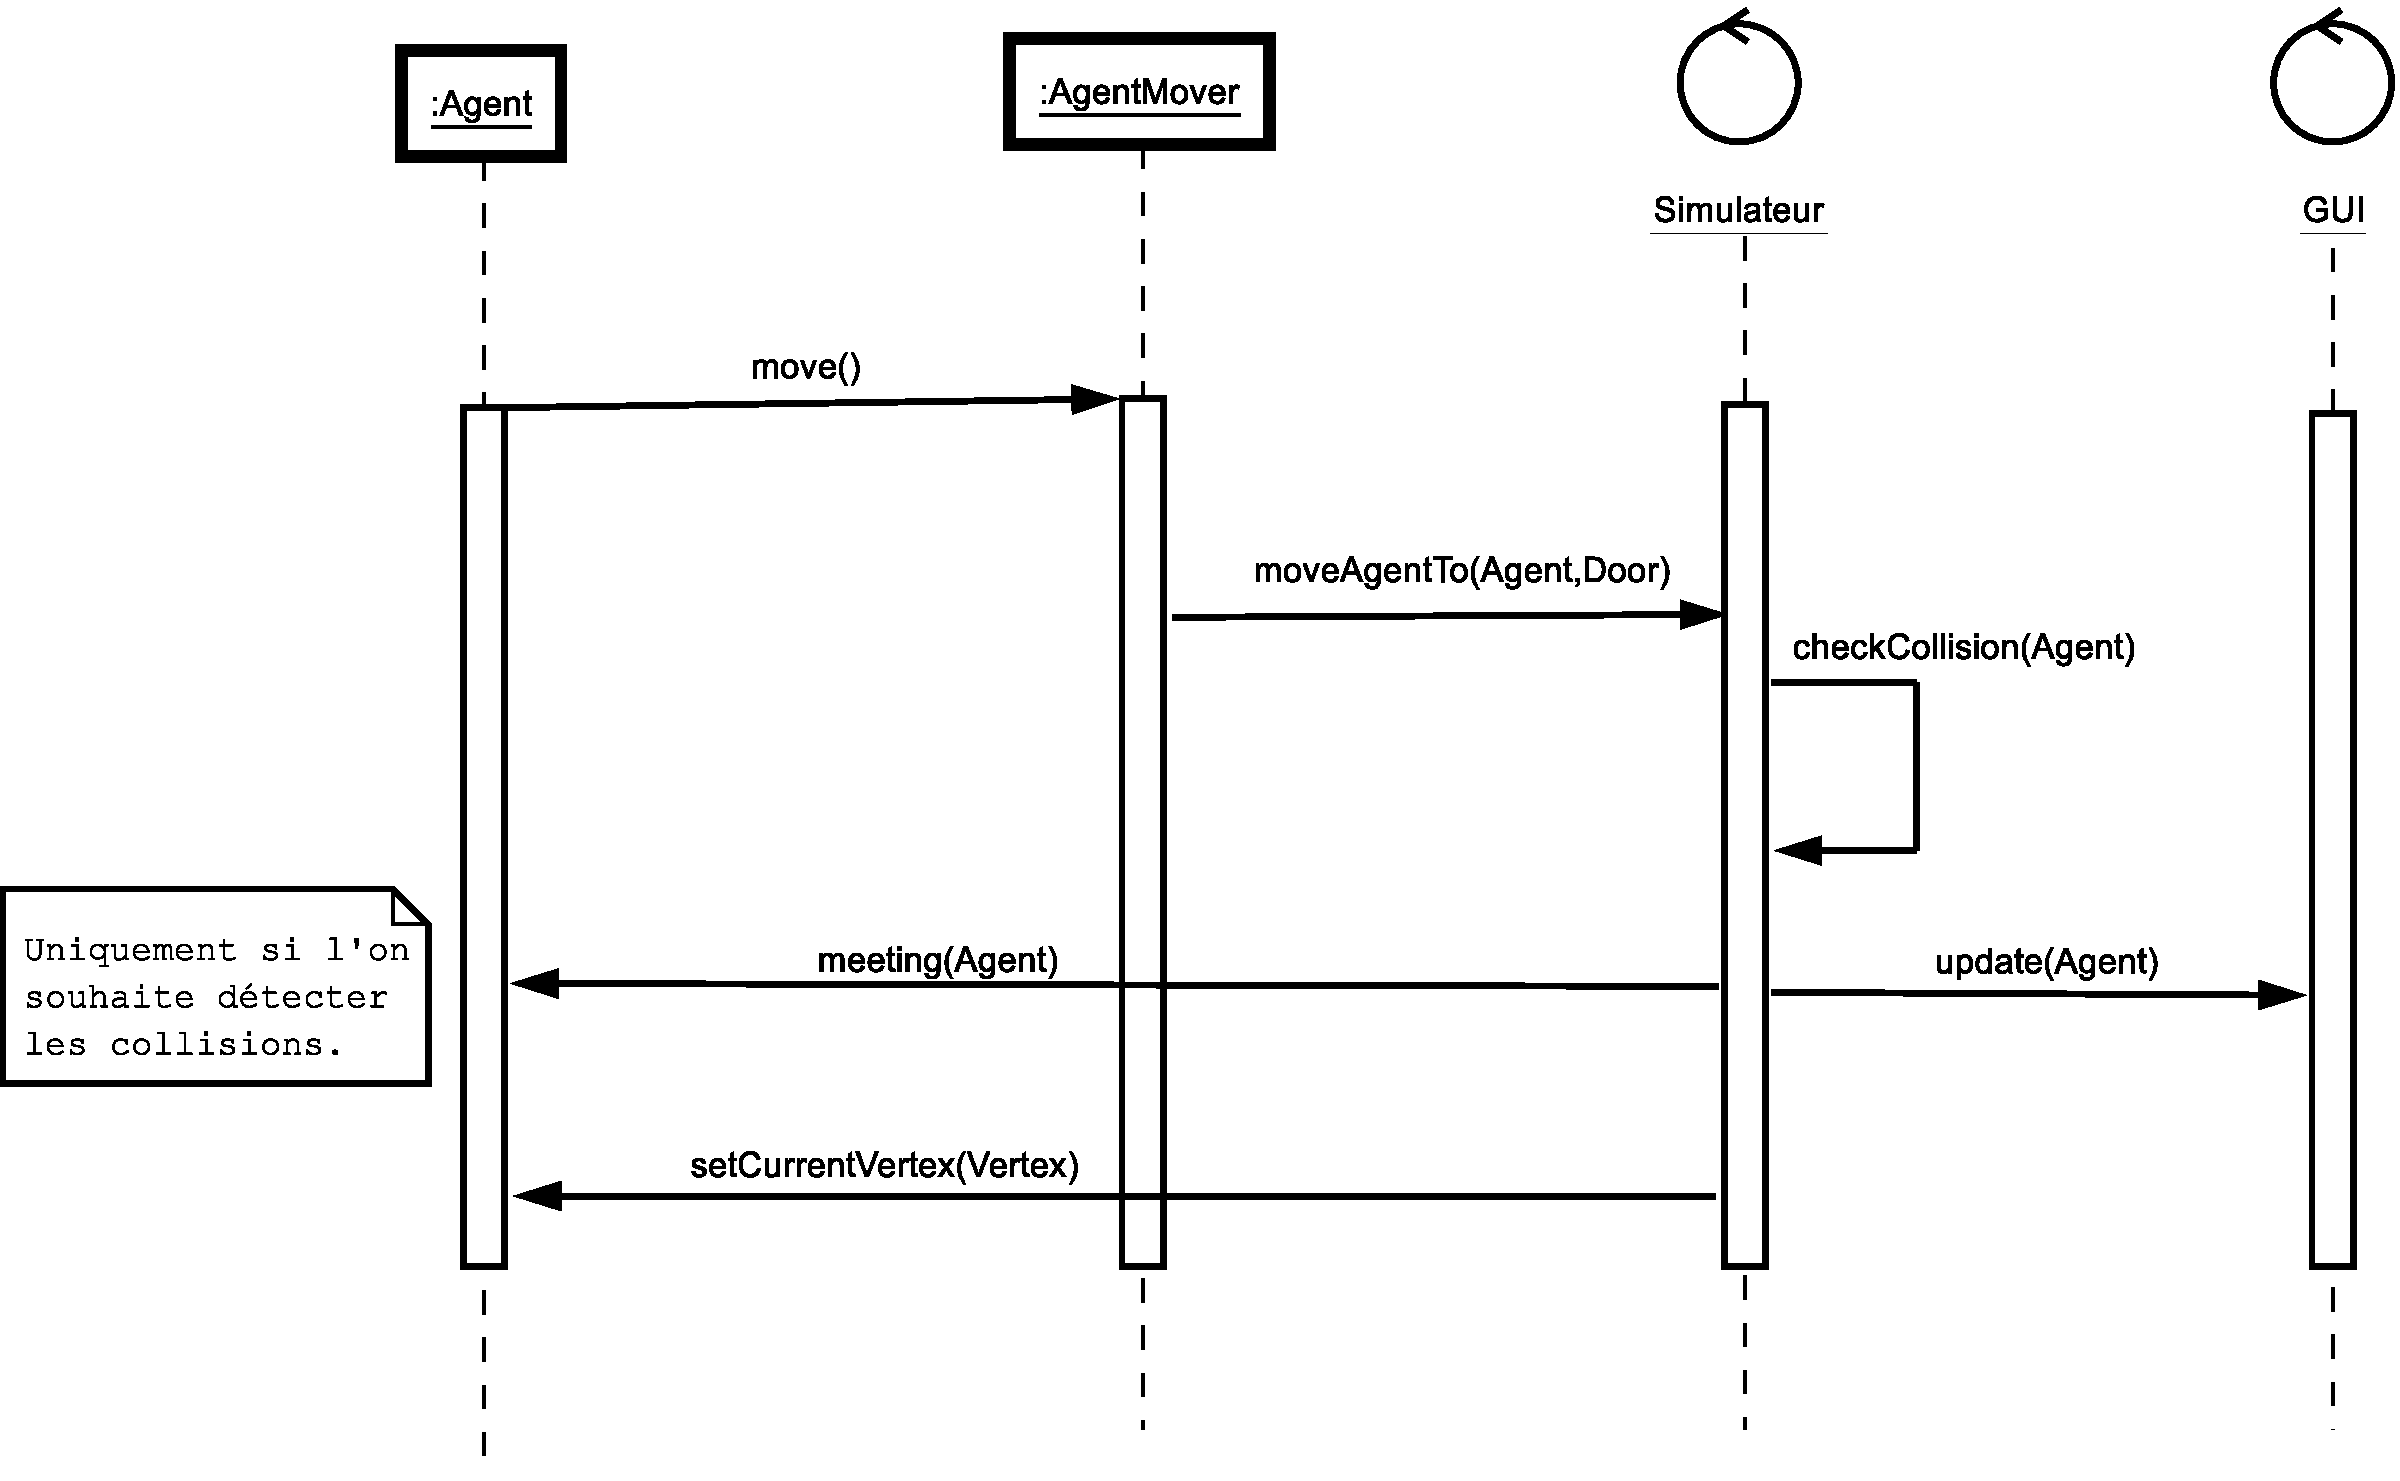
\includegraphics[width=14cm]{seqDeplacement}
  \caption{Sc�nario de d�placement}
  \label{fig:diagramme_seqDeplacement}
\end{figure}

\subsection{Propri�t�s}

Figure   \ref{fig:diagramme_seqProperties}  :   Sc�nario   o�  l'agent
souhaite modifier ou obtenir une propri�t� d'un sommet.

\begin{figure}[h!t]
  \centering
  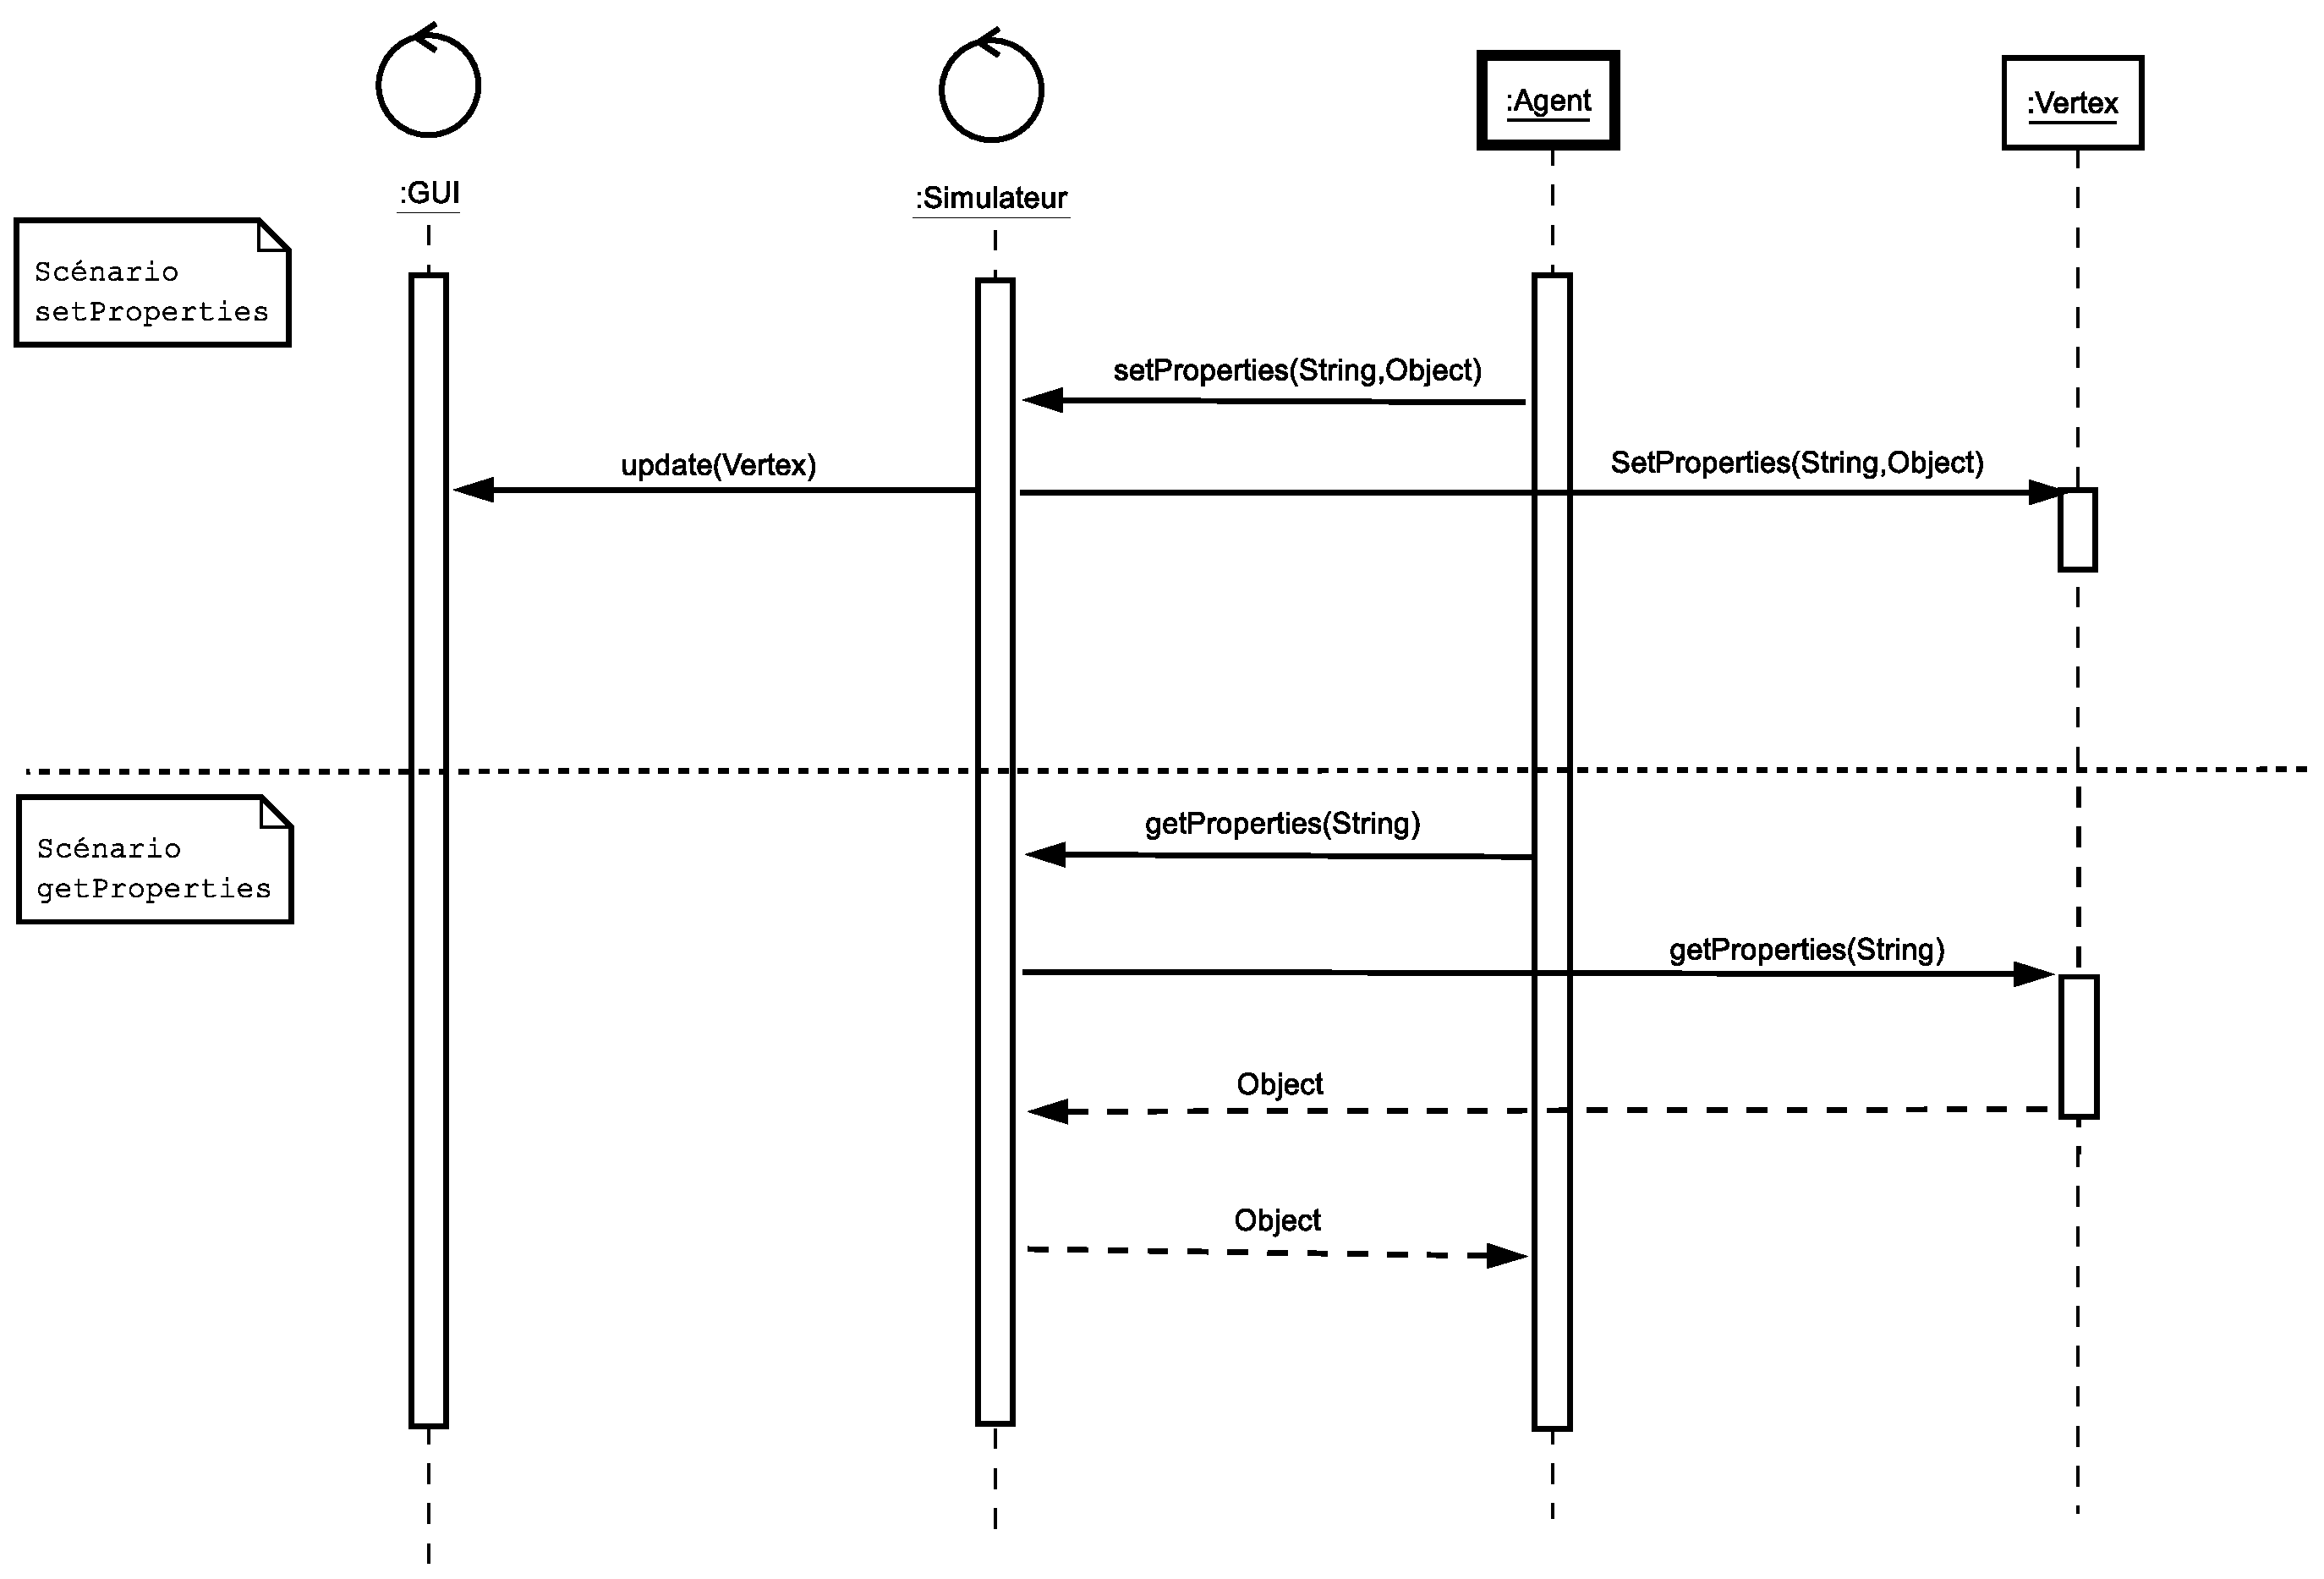
\includegraphics[width=14cm]{seqProperties}
  \caption{Sc�nario de lecture ou �criture d'une propri�t�}
  \label{fig:diagramme_seqProperties}
\end{figure}



\section{Contraintes}

\subsection{Langage et portabilit�}

Notre r�le  est de  d�velopper une extension  de \visidia, �crit  � la
base en  Java :  c'est donc  en Java que  nous �crirons  l'ensemble de
notre  programme,   afin  que  notre  module  s'int�gre   au  mieux  �
l'application.\\

Les  d�veloppeurs ext�rieurs seront  oblig�s de  passer par  notre API
pour concevoir de nouveaux  algorithmes distribu�s, ce qui nous impose
d'�tre compris le plus ais�ment possible par tout le monde. Pour cette
raison,  notre code  sera  r�dig� exclusivement  en  anglais. Le  Java
semble encore un  choix correspondant � notre volont�,  d'une part car
il  s'agit d'un  des langages  les plus  utilis�s actuellement  (si ce
n'est  LE plus  utilis�), d'autre  part  pour sa  portabilit� sur  les
diff�rentes plate-formes existantes.\\

La  documentation quant  �  elle  sera r�alis�e  �  l'aide de  l'outil
Javadoc.\\


\subsection{Standard de codage}

*Utilisation des conventions JAVA :
\begin{itemize}
\item noms des classes commen�ant par une majuscule
\item noms des m�thodes commencent par une minuscule
\item majuscules pour s�parer les diff�rents mots composant un nom 
\item accesseurs commen�ant par 'get'
\item modificateur commen�ant par 'set'\\
\end{itemize}

*Autres standards
\begin{itemize}
\item nom des classes et des m�thodes en anglais
\item reprise au maximum des noms existant
\item utilisation de noms explicites
\item commentaires en anglais style Javadoc
\end{itemize}

\subsection{Licence} 

L'ensemble de notre  programme sera sous licence GNU  GPL (GNU General
Public License)  version 2  ou sup�rieure. Une  version de  la licence
sera disponible en  fran�ais et en anglais dans le  code source, et un
rappel sera effectu� � chaque en-t�te de fichier.


%% Local Variables:
%% mode: latex
%% coding: latin-1
%% TeX-master: "main"
%% End:

%%
\section{Les moyens techniques}

Afin de mener � bien notre projet, nous avons utilis�s un portail �volu� de
d�veloppement fournissant plusieurs outils : le portail berliOs.de \footnote{\url{http://www.berlios.de}}
\\ \newline
Pour am�liorer la communication avec notre client et notre responsable
p�dagogique, nous avons mis en place un wiki sur lequel on pouvait retrouver
toutes les principales informations relatives au projet.\\

\begin{figure}[H]
  \centering
  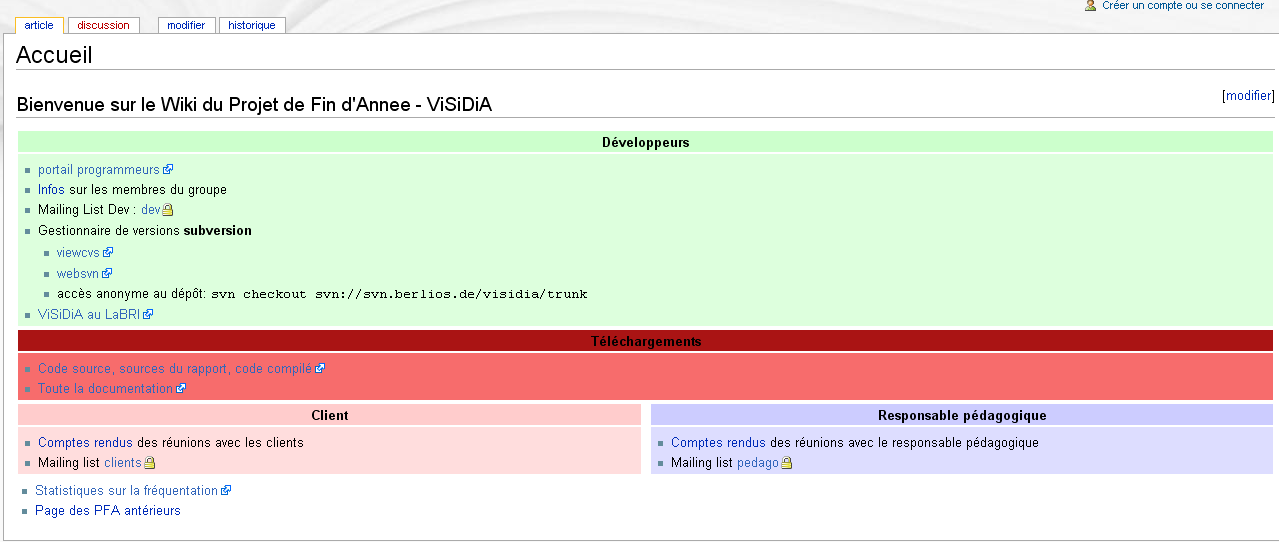
\includegraphics[width=16cm]{images/wiki.png}
  \caption{Le wiki du projet Visidia}
\end{figure}

Nous avons d�ploy�s plusieurs listes de diffusion pour faciliter la communication :
\begin{itemize}
  \item Une liste pour tous les d�veloppeurs
  \item Une liste de diffusion pour communiquer avec le client
  \item Une liste de diffusion pour communiquer avec le responsable p�dagogique \\
\end{itemize}

Nous avons utilis� �galement un gestionnaire de versions, Subversion
, qui nous permet de maintenir les sources de \visidia. 
Les clients ont �galement la possibilit� de
suivre l'avancement du projet et d'acc�der aux sources, gr�ce � deux
interfaces viewcvs  et websvn .  Il est
�galement possible de t�l�charger la derni�re version des sources du
projet:
\begin{verbatim}
svn checkout svn://svn.berlios.de/visidia/trunk
\end{verbatim}


\section{Organisation du travail}

Notre groupe de travail �tant form� de 6 personnes, nous avons d�cid�s de former
trois bin�mes afin de favoriser et optimiser le travail en �quipe. 
De plus la formation de binome permettait de mettre en place le systeme
d�veloppeur/relecteur, et facilite l'appr�hension d'une application comme
\visidia, puisque chacun pouvait expliquer � son partenaire les concepts qu'il avait
saisi pour mututellement enrichir ses connaissances de l'application.\\

Nous nous sommes r�parti le travail de mani�re � faire en sorte, que les binomes
form�s n'ait � se concentrer essentiellement que sur une partie du d�veloppement
de \visidia. Ainsi nous avons eu un binom� charg� d'impl�menter les
fonctionnalit�s relatives aux graphes et un autre celles relatives aux agents.

\section{Avancement du projet}

\begin{figure}[!ht]
  \center
  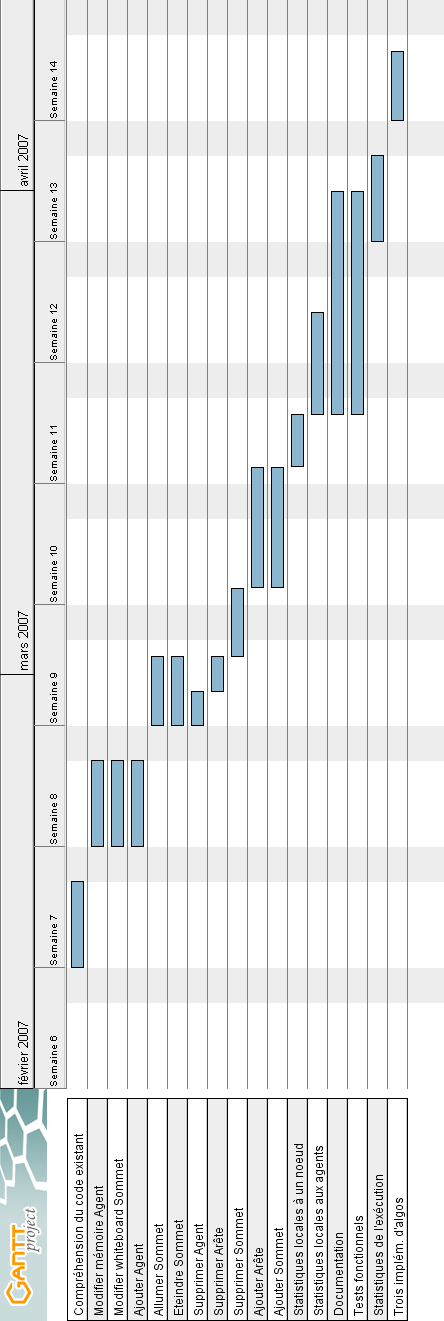
\includegraphics[height=20cm]{images/gantt2.png}
  \caption{Diagramme de Gantt}
\end{figure}
%diagramme de gant a mettre la



\chapter{�volution du syst�me}
%          * Suppositions fondamentales
%          * Adaptations possibles 

Une �volution envisageable de \visidia consisterait � d�velopper un applet java afin de pouvoir utiliser
l'application � l'aide d'un simple navigateur internet.

Il pourrait �tre interressant �galement de r�aliser de la simulation d'algorithmes distribu�s sur de vrais r�seaux de machines physiques.
\chapter{Lexique}

Vous  trouverez  ci-dessous les  d�finitions  relatives aux  principaux
termes et sigles utilis�s dans la r�alisation du cahier des charges.


\begin{description}

\item[Algorithmique distribu�e] : Cette partie de l'algorithmique
s'int�resse aux algorithmes s'ex�cutant sur plusieurs unit�s de calcul
en m�me temps. Le mod�le th�orique d'un r�seau dans ce cadre est un
graphe dont les sommets (ou noeuds) sont des machines ou processeurs
et les ar�tes des connexions.

\item[Agent   mobile]   :   Entit�   autonome   de   calcul   qui   se
d�place \cite{agentBook}.

\item[A.P.I.]   :  Application  Programming  Interface.   Ensemble  de
prototypes   de  fonctions   accessibles   depuis  l'ext�rieur   d'une
biblioth�que. C'est l'interface publique de la biblioth�que.

\item[Door  ou porte]  : une  porte est  une connexion  �  partir d'un
sommet du graphe  vers un autre sommet.  Les  portes sont num�rot�es �
partir de 0.

\item[ENSEIRB]   :    �cole   Nationale   Sup�rieure   d'�lectronique,
Informatique et Radiocommunications de Bordeaux \cite{enseirb}.

\item[Javadoc] :  outil qui  permet de g�n�rer  de la  documentation �
  partir du code source et des commentaires Java.

\item[LaBRI]  :  Laboratoire Bordelais  de  Recherche en  Informatique
\cite{labri}.

\item[PFA]  :  Projet  de  Fin  d'Ann�e. Module  de  programmation  de
  quatri�me semestre  de fili�re informatique �  l'ENSEIRB.  Ce module
  consiste en  l'�laboration d'un  projet sur une  dur�e de 3  mois en
  groupe de 7  � 8 personnes. Il a pour but  de nous familiariser avec
  les m�thodes  de travail  en groupe sur  des projets de  plus longue
  dur�e  et   de  plus  grande   taille  que  ceux  dont   nous  avons
  l'habitude. Dans le cadre du pr�sent projet, les chercheurs du LaBRI
  constituent donc les clients auxquels  on doit rendre des comptes en
  tant que prestataires.

\item[thread  ou processus  l�ger]  :  un thread  est  similaire �  un
  processus : il ex�cute  un ensemble d'instructions. Toutefois, l� ou
  chaque processus  poss�de sa  propre m�moire virtuelle,  les threads
  qui appartiennent au m�me processus p�re partagent un m�me partie de
  sa m�moire virtuelle.

\item[\visidia]   :  Visualization   and  Simulation   of  Distributed
Algorithms ou  Visualisation et Simulation  des Algorithmes Distribu�s
\cite{visidiaLaBRI}.

\end{description}



%% Local Variables:
%% mode: latex
%% coding: latin-1
%% TeX-master: "main"
%% End:
\chapter{Bibliographie}





%% Local Variables:
%% mode: latex
%% coding: latin-1
%% TeX-master: "main"
%% End:


\end{document}
